\documentclass[tikz,border=4pt]{standalone}
% Shared art direction for the "phones" post, after Vagrancy's region art
% (vagrancy/analysis/art/regions.py and data/palette.json "art"): flat fills,
% plum ink lines, a mustard sky, peach and sage. Every colour below is copied
% from that palette so the post and the game look like one hand drew them.
%
% The scenes share a horizon at y=2.6 and the same sky band, so consecutive
% figures read as one continuous walk down the page.
\usetikzlibrary{arrows.meta,calc,decorations.pathmorphing}
\definecolor{ink}{HTML}{3B2A3F}
\definecolor{sky}{HTML}{E9C46A}
\definecolor{skylight}{HTML}{F2DC98}
\definecolor{cloud}{HTML}{F6E7B8}
\definecolor{peach}{HTML}{EBA77C}
\definecolor{peachdark}{HTML}{D98B5C}
\definecolor{cream}{HTML}{F3E6C4}
\definecolor{sage}{HTML}{9DB58A}
\definecolor{sagedark}{HTML}{6F8F66}
\definecolor{olive}{HTML}{B9B566}
\definecolor{teal}{HTML}{79ADA4}
\definecolor{tealdark}{HTML}{4F8580}
\definecolor{slate}{HTML}{6E8494}
\definecolor{stone}{HTML}{C9B79C}
\definecolor{wood}{HTML}{A9774E}
\definecolor{gold}{HTML}{E3B04B}
\definecolor{shadow}{HTML}{5B4A63}
\tikzset{
  ln/.style={draw=ink, line width=0.9pt, line join=round},
  thinln/.style={draw=ink, line width=0.6pt, line join=round},
  lab/.style={font=\sffamily\scriptsize, text=ink, align=center},
  tag/.style={font=\sffamily\scriptsize\bfseries, text=ink, align=center},
}
% A walking figure. #1 x, #2 y, #3 body colour, #4 head tilt in degrees
% (0 upright, negative looking down at a phone).
\newcommand{\walker}[4]{%
  \begin{scope}[shift={(#1,#2)}]
    \filldraw[fill=#3, ln] (-0.13,0) rectangle (0.13,0.52);
    \draw[ln] (-0.09,0) -- (-0.14,-0.28);
    \draw[ln] (0.09,0) -- (0.17,-0.26);
    \begin{scope}[rotate around={#4:(0,0.52)}]
      \filldraw[fill=cream, ln] (0,0.66) circle (0.14);
    \end{scope}
  \end{scope}}

\begin{document}
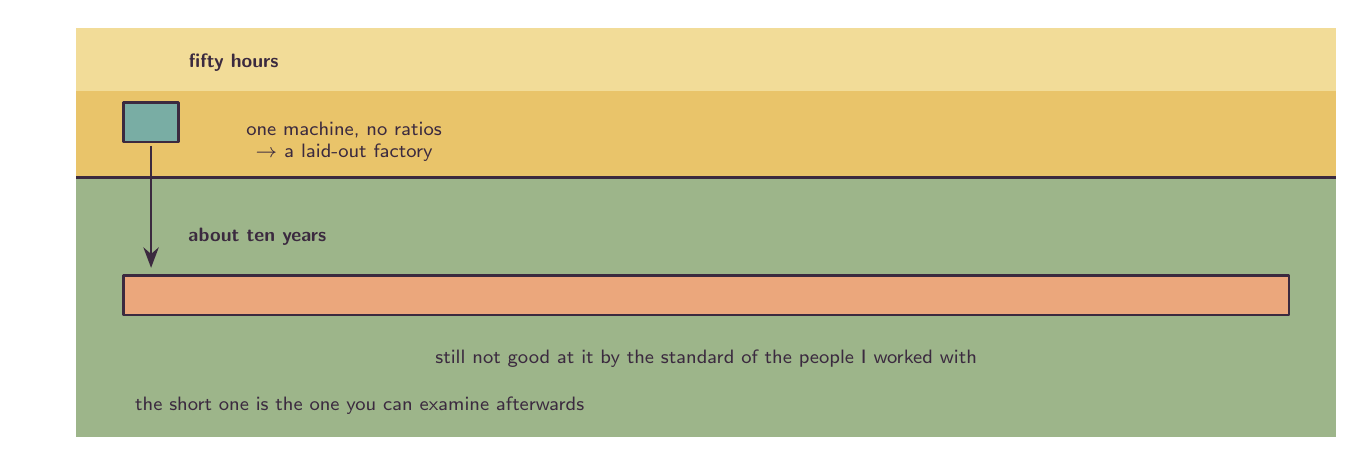
\begin{tikzpicture}[font=\sffamily]
  \fill[sky] (0,3.3) rectangle (16,5.2);
  \fill[skylight] (0,4.4) rectangle (16,5.2);
  \fill[sage] (0,0) rectangle (16,3.3);
  \draw[ln] (0,3.3) -- (16,3.3);
  % The two spans drawn to the same scale, which is the argument: fifty hours
  % is a thing you can finish and look back at, ten years is not.
  \node[tag, text width=5cm] at (2.0,4.75) {fifty hours};
  \filldraw[fill=teal, ln] (0.6,3.75) rectangle (1.3,4.25);
  \node[lab, text width=4.6cm] at (3.4,3.75) {one machine, no ratios \\ $\rightarrow$ a laid-out factory};

  \node[tag, text width=5cm] at (2.3,2.55) {about ten years};
  \filldraw[fill=peach, ln] (0.6,1.55) rectangle (15.4,2.05);
  \node[lab, text width=9.5cm] at (8.0,1.0) {still not good at it by the standard of the people I worked with};

  % The bar for fifty hours, to the same scale, is the small mark at the left.
  \draw[ln, -{Stealth[length=2.6mm]}] (0.95,3.7) -- (0.95,2.15);
  \node[lab, text width=6.4cm] at (3.6,0.4) {the short one is the one you can examine afterwards};
\end{tikzpicture}
\end{document}
